\section{2-D XY model}
\subsection{Single Vortices}
Let us recap where we ended up last class. What has been missing thus far from our discussion of continuous systems is the presence of vortices. We were assuming that we could capture everything with slow variations of spins, but this leaves out configurations like those that appear in Fig. \ref{fig:vortexcharges}. We can define such vortices by looking at:
\begin{equation}
    \oint (\nabla \theta) \cdot d\v{S} = 2\pi n
\end{equation}

We can make vortices that wind more than once, or those that have negative $m$ (antivortices). Since:
\begin{equation}
    \nabla \theta  = -n\nabla \times (\zhat \ln r) \sim \frac{1}{r}
\end{equation}

Let's compute the energy of a vortex.

\begin{equation}
    \beta \mathcal{E}_m = \beta \mathcal{E}_0(a) + \frac{1}{2}\kappa\int_a^L d^2x (\nabla \theta)^2 = \beta \mathcal{E}_0(a) + \pi \kappa n^2 \ln(L/a)
\end{equation}
which diverges in the system size. This may suggest that we might not have any vortices - but this is not the case. Let's look at the partition function:
\begin{equation}
    Z(n) \approx \left(\frac{L}{a}\right)^2 e^{-\beta \mathcal{E}_0(a)} e^{-\pi \kappa n^2 \ln(L/a)}
\end{equation}
The $\mathcal{E}_0(a)$ is like the chemical potential, and we can call its exponential the fugacity. We have:
\begin{equation}
    Z(n) \approx y_0(a) \left(\frac{L}{a}\right)^{2 - \pi\kappa n^2}
\end{equation}
Let us also remember that $\kappa \propto \frac{1}{T}$. So, above $T_c \sim \frac{\pi}{2}n^2$ is where the vortices proliferate (look at the term in the partition function). Although the energy contribution is infinite, the entropic gain wins out at this temperature.

\subsection{Pairs of Vortices}
This was a single vortex; there are also pairs of vortices, which is what we will have to pay attention to. Consider a vortex anti-vortex pair at distance $d$. We then find:
\begin{equation}
    (\nabla \theta) \sim d \nabla\left(\frac{\v{r} \times \v{z}}{r}\right) \sim \frac{1}{r^2}
\end{equation}
These have finite energy, and act like a Coloumb gas.

Consider a flow, which we treat by looking at a sum of a rotational and irrotational part.
\begin{equation}
    \v{u}(\v{r}) = \nabla \theta 
\end{equation}
One part is curl free (this is the piece without vortices):
\begin{equation}
    (\nabla \times u_0) = 0 \implies u_0 = \nabla \phi
\end{equation}
Then:
\begin{equation}
    u = u_0 - \nabla \times (\v{z} \psi)
\end{equation}
where if we consider the contribution from vortices:
\begin{equation}
    \oint \v{u} \cdot d\v{S} = 2\pi \zhat \sum_i n_i \delta(r - r_i)
\end{equation}
Then:
\begin{equation}
    \nabla \times \v{u} = \zhat \nabla^2 \psi
\end{equation}
We can then see:
\begin{equation}
    \nabla^2 \psi = 2\pi \sum_i n_i \delta(r - r_i)
\end{equation}
So then:
\begin{equation}
    \psi(r) = \sum_i n_i \ln(\abs{r - r_i})
\end{equation}
Having written the field as this, let us compute the energy:
\begin{equation}
    \beta H = \frac{1}{2}\kappa \int d^2r \left[(\nabla \phi)^2 - 2(\nabla \phi) \cdot \nabla(\zhat \psi) + (\nabla \times \zhat\psi)^2\right]
\end{equation}
The middle term vanishes via integrating by parts. The first term is familiar. The third term looks like:
\begin{equation}
    (\nabla \times \zhat\psi)^2 = \left(-\dpd{\psi}{x}, \dpd{\psi}{y}, 0\right)^2 = (\nabla \psi)^2
\end{equation}
We then have (through an integration by parts):
\begin{equation}
    \beta H_1 = \kappa \int d^2r (\nabla \psi)^2 = -\frac{\kappa}{2}\int d^2 r \psi \nabla^2 \psi = -\frac{\kappa}{2}\int d^2r (\sum_i n_i \ln(\abs{r - r_i}))(\sum_j 2\pi n_j \delta(r - r_j))
\end{equation}
which we can now use to define the correlation function:
\begin{equation}
    \beta H_1 = -\frac{\kappa}{2}\int d^2r \sum_{i\neq j} n_i n_j C(r_i - r_j)
\end{equation}
where:
\begin{equation}
    C(r_i - r_j) = \frac{\ln(\abs{r_i - r_j})}{2\pi}
\end{equation}
and we exclude a vortex interacting with itself.

\subsection{Transitions}
Now, we may go back and write down the full partition function:
\begin{equation}
    Z = \int \mathcal{D}\phi e^{-\frac{\kappa}{2}\int (\nabla \phi)^2}\sum_{r_k}\int d^2r_k e^{-\sum_i \beta\mathcal{E}_0(r_i) + 4\pi^2\kappa \sum_{ij} n_i n_j C(r_i - r_j)}
\end{equation}
The first term corresponds to spin waves, and the second corresponds to vortices, so we can write:
\begin{equation}
    Z = Z_{SW}Z_{\text{vort}}
\end{equation}
We also constrain the configuration to that which where $\sum_i n_i = 0$, and restrict to $n_i = \pm 1$. To make the connection with charges more clear, we replace $n_i$ with $q_i$. We then study:
\begin{equation}
    Z_v = \sum_{N=0}^\infty (y_0)^N \int \prod_{k=1}^N d^2r_k \exp(4\pi^2\kappa\sum_{ij}q_iq_jC(r_i - r_j))
\end{equation}

Suppose the fugacity is small, such as in a metal-insulator. Then, $y_0$/the fugacity is small ($y_0$ can be thought to be controlling the density), and we should see that the vortices bind in pairs. Here, $C(x) \to C(x)/\mathcal{E}$. There is another limit where $y_0$ is large, and then the bound pairs of charges start to overlap highly, so much so that the charges become unbound. This is the plasma phase. and we see $C(x) \sim e^{-x/\xi}$. 

We have:
\begin{equation}
    Z \sim y_0(a) \left(\frac{L}{a}\right)^{2-\pi\kappa} \to y_0(ba)\left(\frac{L}{ba}\right)^{2 - \pi \kappa}
\end{equation}
where we rescale such that the partition function remains invariant. Then if we make $b \sim e^{-\delta l}$:
\begin{equation}
    \dod{y_0}{l} = (2 - \pi \kappa)y_0
\end{equation}
The $x = 2 - \pi \kappa$ parameter tells us whether vortices are relevant or not.

We then assert:
\begin{equation}
    \dod{x}{l} = Ay_0^2
\end{equation}

Which gives rise to the flow diagram:

\begin{figure}[htbp]
    \centering
    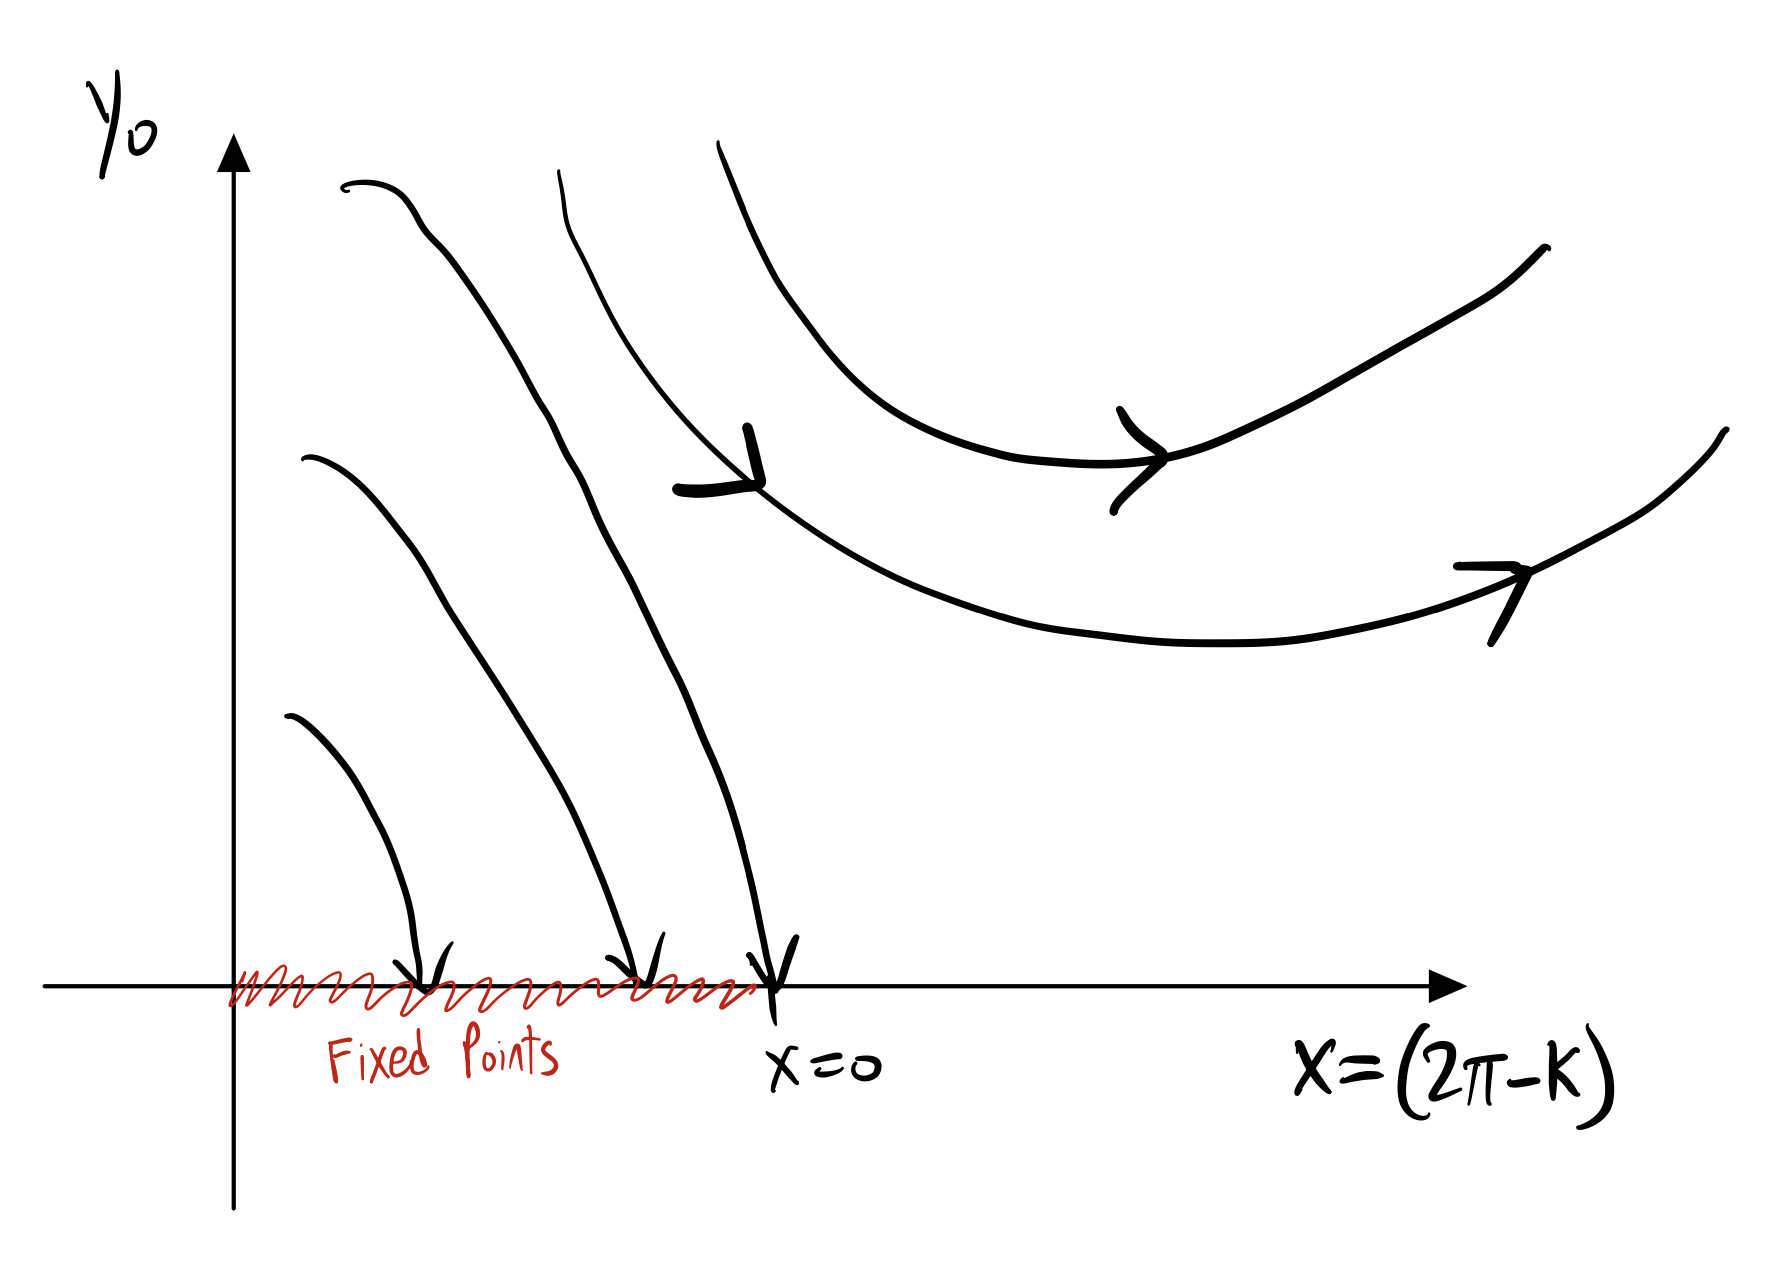
\includegraphics[scale=0.3]{Lectures/Figures/xymodelflow.png}
    \caption{Flows of fugacity and stiffness in the 2-D XY model, corresponding to 2 different phases with differing behaviour of vortices.}
    \label{fig:xymodelflow}
\end{figure}

So we have two regimes, one where vortices are irrelevant and another where they proliferate. There is a separatrix line which is the dividor between whether we flow to no vortices or proliferation. We can say this defines a physical transition temperature, known as the Berezinskii-Kosterlitz-Thouless temperature.

Lastly, let us think about what the correlation functions look like:
\begin{equation}
    \avg{\psi(r)\psi(0)} = \frac{1}{r^{1/2\pi\kappa}}
\end{equation}
Notice that this power law varies. When we get to $k = 2/\pi$, at that point the correlator goes as $\sim \frac{1}{r^{1/4}}$. But, everywhere along the line of $x = 0$ fixed points there is a (continously varying) power law (i.e. each point along the line has a different critical exponent), up until $r^{-1/4}$, at which afterwards it becomes a short-range correlator $e^{-r/\xi}$ which exponential decay. This means, at the transition temperature, there is a jump in physical properties.

\subsection{Polarizability + Looking ahead}

Suppose we add an external field:
\begin{equation}
    H = H_0 + \v{E} \cdot \sum_{\v{R}} \v{R} \cdot n(R)
\end{equation}
Suppose now we want to compute the dielectric function:
\begin{equation}
    \chi_{ij} = \frac{\partial f}{\partial E_i \partial E_j} \sim \sum \sum_{\v{R}}R^2\avg{n(R)n(0)} = \int dR R^3 e^{-2\pi\kappa \ln(R)} = \int_a^L dR R^{3-2\pi\kappa} L^{4-2\pi\kappa}
\end{equation}
which depending on $\kappa$ either diverges or vanishes. It diverges when $\kappa = 2/\pi$. This connects back up to the correlation function above.

Next day, we move to disorder and randomness. Everything we have talked about thus far assumes a perfect medium and translational invariance. We will now break this. This is both relevant in a practical sense (every physical system has disorder of some form), and also inherently interesting problems with disorder, e.g. frustration. We could consider models with sufficient randomness such that the spins have confusion about their orientation, then we can get systems that act glassy - they freeze into a disorder state. There is a sharp transition from a slowly-flowing material to something that freezes; this is called a spin glass, and we will talk about the infinite-range spin-glass, which we will be able to solve exactly (the Parisi solution - he won a Nobel prize for this)! Interestingly, these kinds of models allow you to store information/use them as a physical memory, which was John's Hopfield's idea. Rapidly coming out of this was how one ``learns'' via tuning parameters, the simplest of which is the Boltzmann machine. Of course, this was the Nobel prize in physics this year.